\section{Evaluation}
	\label{sec:evaluation}
	
	In this section, we assess the efficiency of our algorithm through case studies coming from the DREAM4 challenge \cite{prill2011crowdsourcing}.

	DREAM challenges are annual reverse engineering challenges that provide biological case studies.
	In this paper, we focus on the datasets coming from DREAM4.
	The input data that we tackle here consists of the following:
	5 different systems each composed of 100 genes, all coming from E. coli and yeast networks. For every such system,
	the available data are the following: (i) 10 time series data with 21 time points and 1000 is the duration of each time series; (ii) steady state for wild type;
	(iii) steady states after knocking out each gene;
	(iv) steady states after knocking down each gene (i.e. forcing its transcription rate at 50\%);
	(v) steady states after some random multifactorial perturbations. We processed all the data.
	Here, we focus on the management of time series data.

\subsection{Settings}

	Each time serie includes different perturbations that are maintained all time along during the first 10 time points and applied to at most 30 genes.
	In this setting, a perturbation means a significant increase or decrease of the gene expression.
	%
	In the raw data of the time series, gene expression values are given as real number between 0 and 1.
	To apply our approach, we chose to discretize those data into two to six qualitative values.
	Each gene is discretized in an independent manner, with respect to the following procedure:
	we compute the average value of the gene expression among all data of a time series,
	then the values between the average and the maximal/minimal value are divided into as many levels.
	Discretizing the data according to the average value of expression is expected to reduce the impact of perturbation on the discretization and thus on the model learned.
	But in this experiment our goal is to assess the scalability of our approach in practice rather than evaluating the model learned when facing perturbated data.
	Figure \ref{fig:run_time} shows the impact of both indegree per action and discretization level on run time.

\subsection{Results}

	\begin{figure} \centering
	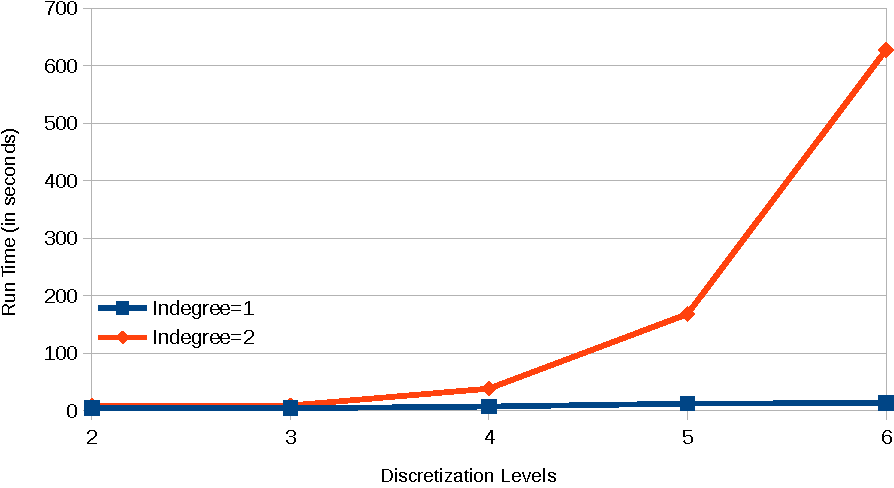
\includegraphics[width=0.32\linewidth]{images/net1}
	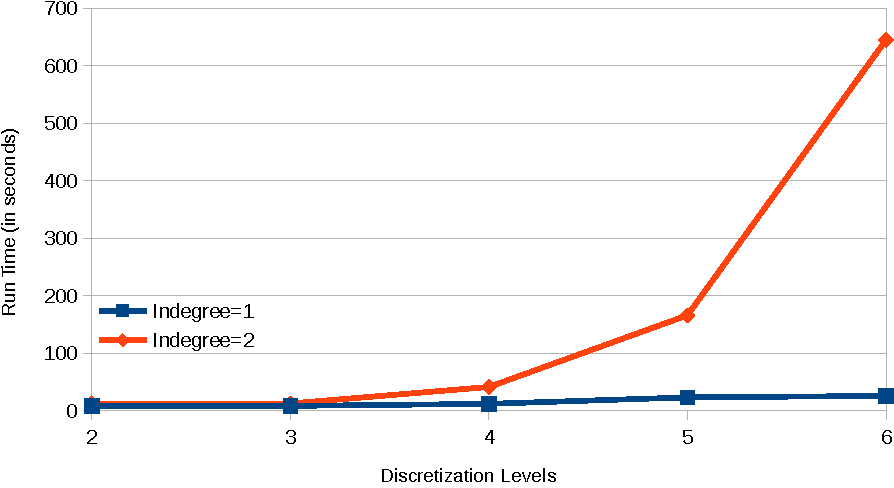
\includegraphics[width=0.32\linewidth]{images/net2}
	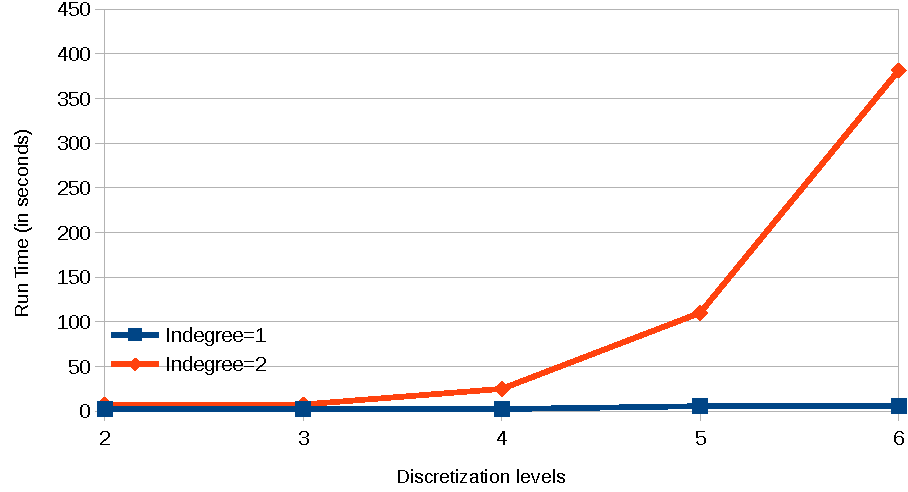
\includegraphics[width=0.32\linewidth]{images/net3}
	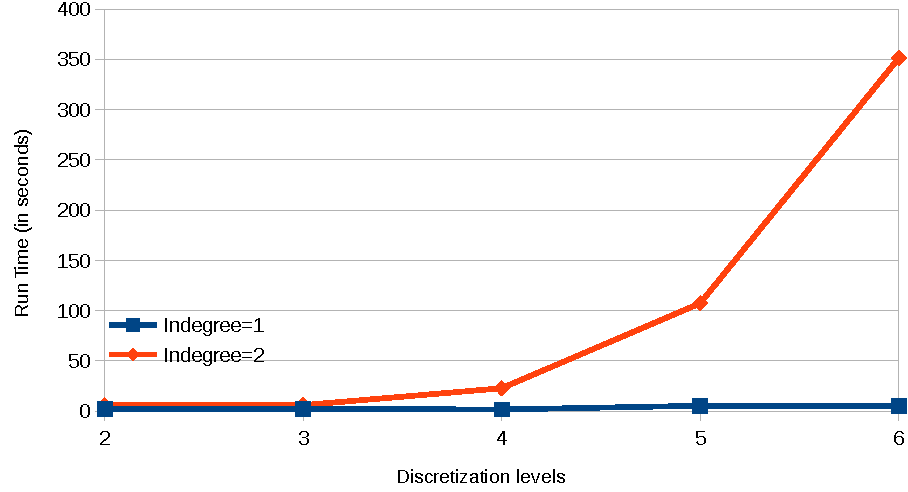
\includegraphics[width=0.33\linewidth]{images/net4}
	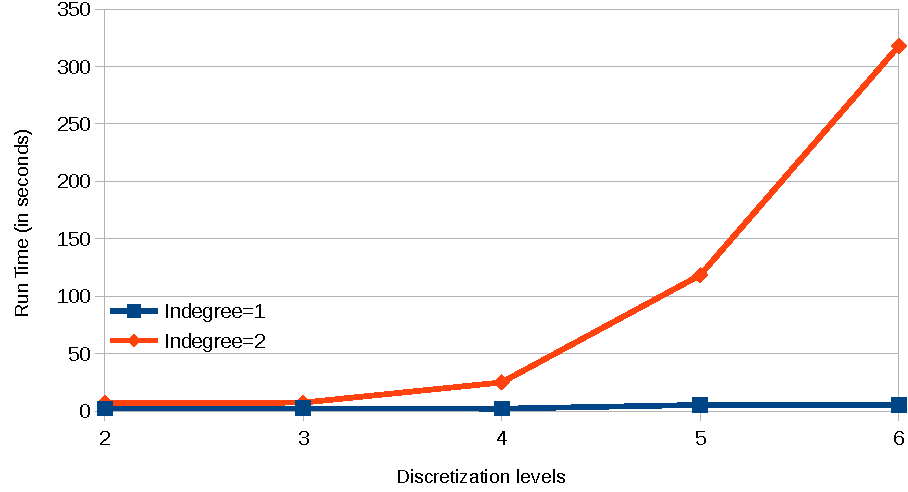
\includegraphics[width=0.33\linewidth]{images/net5}
	\label{fig:run_time}
	\caption{Evolution of run time on processing different model time series data from DREAM4 varying indregree of actions and discretization levels. These tests were performed on processor: 3 GHz Intel Core i7 with 16 Go of RAM. }
	\end{figure}

	In the results optained from the experimentations of our algorithm on the time series data of the DREAM4 we can see the exponential influence on the run time of indegree of action considered as well as the level of discretization chosen for all the 5 different networks.
	But it also shows that in practice our approach can tackle big network, here 100 genes.
	It is important to note that here the real influences are given as background knowledge, 
	thus it greatly reduce the quantity of action generated to explain each change.
	Without knowledge about those influence, the algorithm can be run considering that all gene can be influences by every others.
	But here, the quantity of combination of influences is so big that processing only one time series discretized into two levels of expression with an indegree of two takes more that 12 hours to process. In practice, on big network, accessing to information about genes influence is crucial for the efficiency of the method.

%\textcolor{red}{COMMENT Tony: Faudrais testé en augmentant le nombre de time points si possible. Egalement avec un indegree de 3, 4 jusqu'a ce que ça soit trop long.}
